\begin{frame}
  Egészítsük ki a \texttt{Matrix} osztályt olyan konstruktorral, ami egy \texttt{rows} sorból és \texttt{cols} oszlopból álló 
mátrixot véletlenszerűen feltölt \texttt{min} és \texttt{max} közé eső értékekkel!
  \begin{exampleblock}{\textattachfile{12/matrix12.h}{12/matrix12.h} %
    (\textattachfile{12/CMakeLists.txt}{12/CMakeLists.txt})}
    \lstinputlisting[style=cpp,linerange={8-9},numbers=left,firstnumber=8]{12/matrix12.h}
    \lstinputlisting[style=cpp,linerange={13-14},numbers=left,firstnumber=13]{12/matrix12.h}
    \lstinputlisting[style=cpp,linerange={27-27},numbers=left,firstnumber=27]{12/matrix12.h}
  \end{exampleblock}
\end{frame}

\begin{frame}
  \begin{exampleblock}{\textattachfile{12/matrix12.h}{12/matrix12.h}}
    \scriptsize
    \lstinputlisting[style=cpp,linerange={29-41},numbers=left,firstnumber=29]{12/matrix12.h}
  \end{exampleblock}
  A \kiemel{BAD} sor kizárólag tesztelési célokat szolgál, hogy néha intervallumon kívüli értékek kerüljenek a mátrixba.
\end{frame}

\begin{frame}
  \begin{exampleblock}{\textattachfile{12/matrix12test.cpp}{12/matrix12test.cpp}}
    \scriptsize
    \lstinputlisting[style=cpp,linerange={90-105},numbers=left,firstnumber=90]{12/matrix12test.cpp}
  \end{exampleblock}
\end{frame}

\begin{frame}
  \begin{itemize}
    \item Tesztkészlet \texttt{N}-szeri ismétlése. Negatív értékre az örökkévalóságig ismétel. \\ 
      \texttt{{-}-gtest\_repeat=N}
    \item Leállás az első olyan tesztkészlet iterációnál, ami hibát talált. Debuggerből futtatva a teszteket a memória tartalma 
ellenőrizhető. \\ \texttt{{-}-gtest\_break\_on\_failure}
    \item Tesztesetek szűrése: csak akkor fut le egy teszteset, ha létezik olyan pozitív, de nem létezik olyan negatív minta, 
amire illeszkedik. A negatív minták elhagyhatóak. A pozitív mintákat a 
negatívaktól \kiemel{-} választja el. A \kiemel{*} tetszőleges karakterláncra illeszkedik, a \kiemel{?} egy tetszőleges 
karaktert helyettesít. \\ \texttt{{-}-gtest\_filter=poz1:poz2:...:pozN-neg1:neg2:...:negN}
    \item Tesztkészletek és -esetek listázása \\ \texttt{{-}-gtest\_list\_tests}
  \end{itemize}
  Egyes beállítások környezeti változókon keresztül is módosíthatóak.
\end{frame}

\begin{frame}[fragile]
  \begin{block}{Milyen teszteseteink vannak?}
    \tiny
    \begin{verbatim}
wajzy@lenovo:~/Dokumentumok/gknb_intm006/GKxB_INTM006/12/build$ ./matrix_test --gtest_list_tests
Running main() from /home/wajzy/Dokumentumok/gknb_intm006/GKxB_INTM006/12/build/_deps/googletest-src/googletest/src/
  gtest_main.cc
MulTest.
  meaningful
  equality
  rounding
  randomized
MatrixTest.
  print
  toString
  toCString
\end{verbatim}
  \end{block}
\end{frame}

\begin{frame}
  \begin{itemize}
    \item Minden tesztkészlet összes tesztesetének futtatása \\ \texttt{./runTests} \\ \texttt{./runTests 
{-}-gtest\_filter=*}
    \item Csak a \texttt{MulTest} tesztkészlet futtatása \\ \texttt{./runTests {-}-gtest\_filter=MulTest.*}
    \item Az összes \kiemel{r} betűt tartalmazó teszt futtatása, kivéve a \kiemel{String}-et tartalmazókat és 
\texttt{MulTest.rounding}-ot, azaz \texttt{randomized} és \texttt{print} futtatása \\ \texttt{./runTests 
{-}-gtest\_filter=*r*-*String:MulTest.rounding}
    \item Csak a \texttt{randomized} futtatása 100-szor \\ \texttt{./runTests {-}-gtest\_filter=MulTest.randomized 
{-}-gtest\_repeat=100}
  \end{itemize}
\end{frame}
  
\begin{frame}
  \begin{itemize}
    \item Teszteredmények fájlba mentése. Tesztismétlés esetén csak az utolsó iteráció eredményét tartalmazza. 
Alapértelmezett kimenet: \texttt{test\_detail.xml} Ha \kiemel{kimenet} egy mappa, mindig új nevet választ a felülírás 
elkerülésére. \\ \texttt{{-}-gtest\_output=xml<:kimenet>} \\ \scriptsize
    Pl. \texttt{./runTests {-}-gtest\_filter=MulTest.randomized {-}-gtest\_output=xml:egysegteszt.xml}
  \end{itemize}
  \begin{block}{\textattachfile{12/build/egysegteszt.xml}{12/build/egysegteszt.xml}}
    \resizebox{\textwidth}{!}{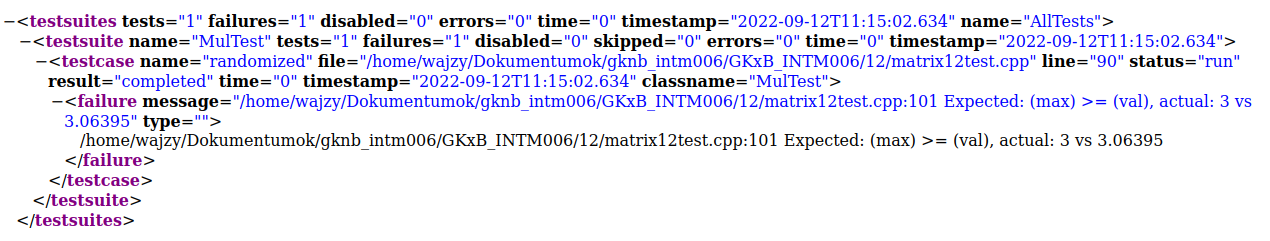
\includegraphics{./xmlout.png}}
  \end{block}
  \begin{itemize}
    \item Az XML megjeleníthető különféle eszközökkel, pl. %
\hiv{\href{https://wiki.jenkins.io/display/JENKINS/xUnit+Plugin}{Jenkins/xUnit}}-tal
  \end{itemize}
\end{frame}